 

\section*{Aufgabe 1: \emph{Zufallszahlen verschiedener Verteilungen}}

\begin{itemize}
\item[a)] Wahrscheinlichkeit zwischen $\frac{1}{2}$ und $\frac{1}{3}$ \\

\[
P\left(A\right) - P\left(B\right)
\]
\[
P\left(x \le \frac{1}{2}\right) - P\left(x \le \frac{1}{3}\right)
\]

Bei einer Gleichverteilung ist die summierte Wahrscheinlichkeit gleich dem Grenzwert.

\[
= \frac{1}{2} - \frac{1}{3} = \frac{3}{6} - \frac{2}{6} = \frac{1}{6}
\]
 \\

\item[b)] Wahrscheinlichkeit von $\frac{1}{2}$ \\

\[
P(A) = \frac{k}{n} = \frac{Günstige Fälle} {Mögliche Fälle}
\]

Wir betrachten eine Gleichverteilung im Intervall $[0,1]$ reeller Zahlen.

Günstiger Fall, Wert $\frac{1}{2}: 1$ \\
Mögliche Fälle: unendlich
\[
\frac{1}{\infty} = 0
\]
\\

\item[c)] Wahrscheinlichkeit von $\frac{1}{2}$ in einem Zufallsgenerator auf dem Computer \\

Um die Wahrscheinlichkeit eines exakten Wertes in einem Zufallsgenerator auf einem
Computer zu bestimmen, pr\"ufen wir, ob diese Zahl auch als bin\"are Gleitkommazahl darstellbar ist.
Wir betrachten den Wert $\frac{1}{2}$, zun\"achst die erste Bin\"arstelle:

\[
 2^{-1} = 1,
\]

fuer alle weiteren Binärstellen gilt

\[
2^{-2} = 2^{-3} = ... = 2^{-23} = 0
\]

Gehen wir von einer theoretischen perfekten Gleichverteilung auf einem Computer aus, 
so hat man einen günstigen Fall zu $2^{23}$ möglichen Fällen.
Die Wahrscheinlichkeit $\frac{1}{2}$ zu treffen ist somit

\[
P\left(\frac{1}{2}\right) = \frac{1}{2^{23}} =\frac{1}{8388608}
\]


Nutzt man nun die Zufallsgeneratoren von Numpy oder ROOT, so sollte unter rund $10000000$ Ereignissen
 der gesuchte exakte Wert sein. Wir haben dies mit der doppelten Anzahl von Zufallszahlen 
und der Verwendung von numpy.random und ROOT.TRandom durchlaufen lassen. 
Das Ergebnis ist in Bild 1 zu sehen.
 \\
\begin{figure}[htbp]
	\centering
	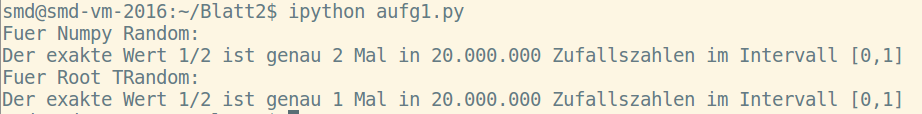
\includegraphics[width=0.7\textwidth]{Gleichvert1zu2.png}
	\caption{Haeufigkeit Zufallszahlen}
\end{figure}
 \\

\item[d)] Wahrscheinlichkeit von $\frac{2}{3}$ in einem Zufallsgenerator auf dem Computer \\

Der Wert $\frac{2}{3}$ l\"asst sich nicht exakt als bin\"are Gleitkommazahl darstellen,
somit ist es einem Zufallsgenerator mit binaeren Gleitkommazahlen nicht m\"oglich,
den Wert exakt darzustellen. Die Berechnung ist in Bild 2 zu sehen. 
Die Addition von jedem ungeraden Exponenten n\"ahert den exakten Wert an, 
jeder gerade Exponent wird \"ubersprungen, da sonst die $\frac{2}{3}$  \"uberschritten werden.

\begin{figure}[htbp]
	\centering
	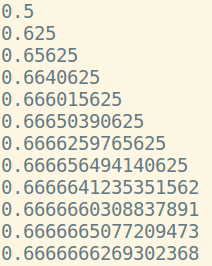
\includegraphics[width=0.4\textwidth]{Binaer2zu3.png}
	\caption{Berechnung im Binaersystem}
\end{figure}


\end{itemize}
\section*{Aufgabe 2: \emph{Zufallszahlengeneratoren}}

Zufallszahlengenerator mit
\begin{equation}
x_n=(ax_{n-1}+b) \text{ mod } m .
\end{equation}

\begin{itemize}


\item[a)] $a=1601$, $b=3456$, $m=10000$.
\item[b)] Das Ergebnis hängt nur vom Startwert ab, wenn dieser nicht durch andere linear kongruente Zufallsgeneratoren erzeugt wird.
\begin{figure}
\centering
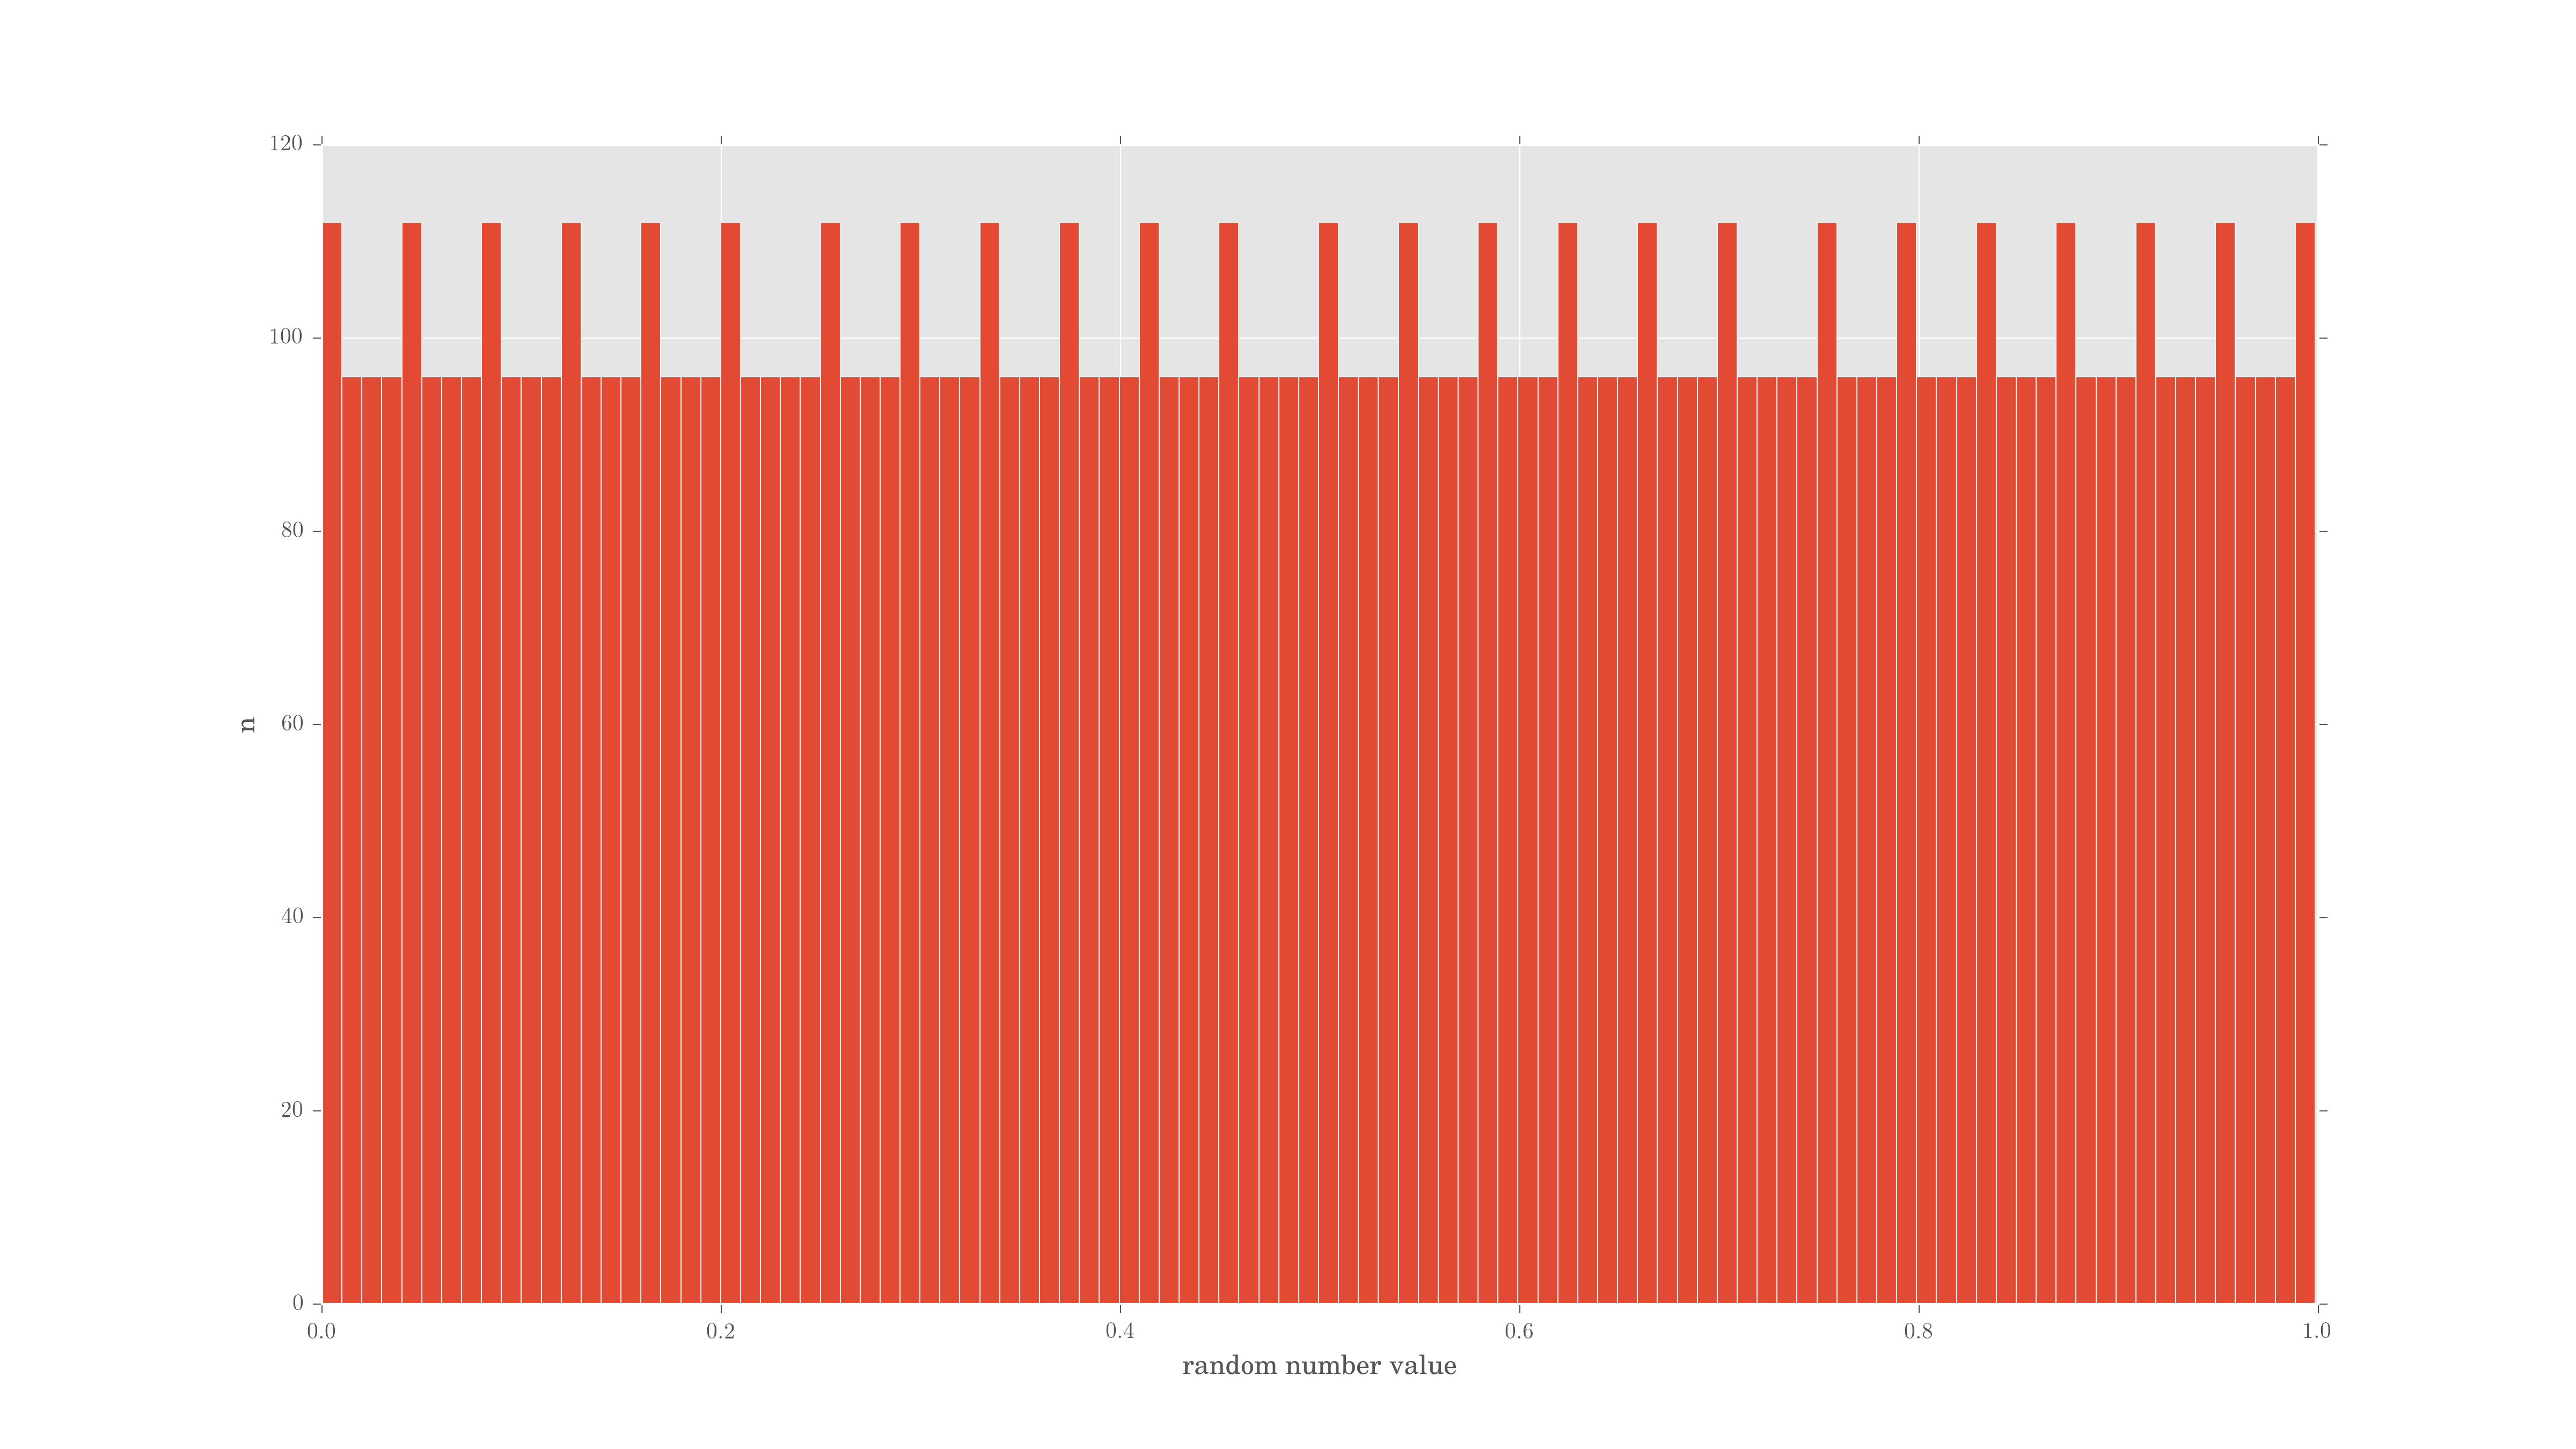
\includegraphics[width=\textwidth]{linear_kongruent_random_numbers.png}
\caption{$10000$ Zufallszahlen, erzeugt mit dem in Aufgabenteil a) programmierten Zufallszahlengenerator.}
\label{fig:2b}
\end{figure}
\item[c)] In den Histogrammen sind eindeutig Strukturen (Linien oder Ebenen) zu erkennen. Dies deutet darauf hin, dass Zahlen von den vorher generierten Zahlen abhängen und nicht komplett gleichverteilt sind.
\begin{figure}
\centering
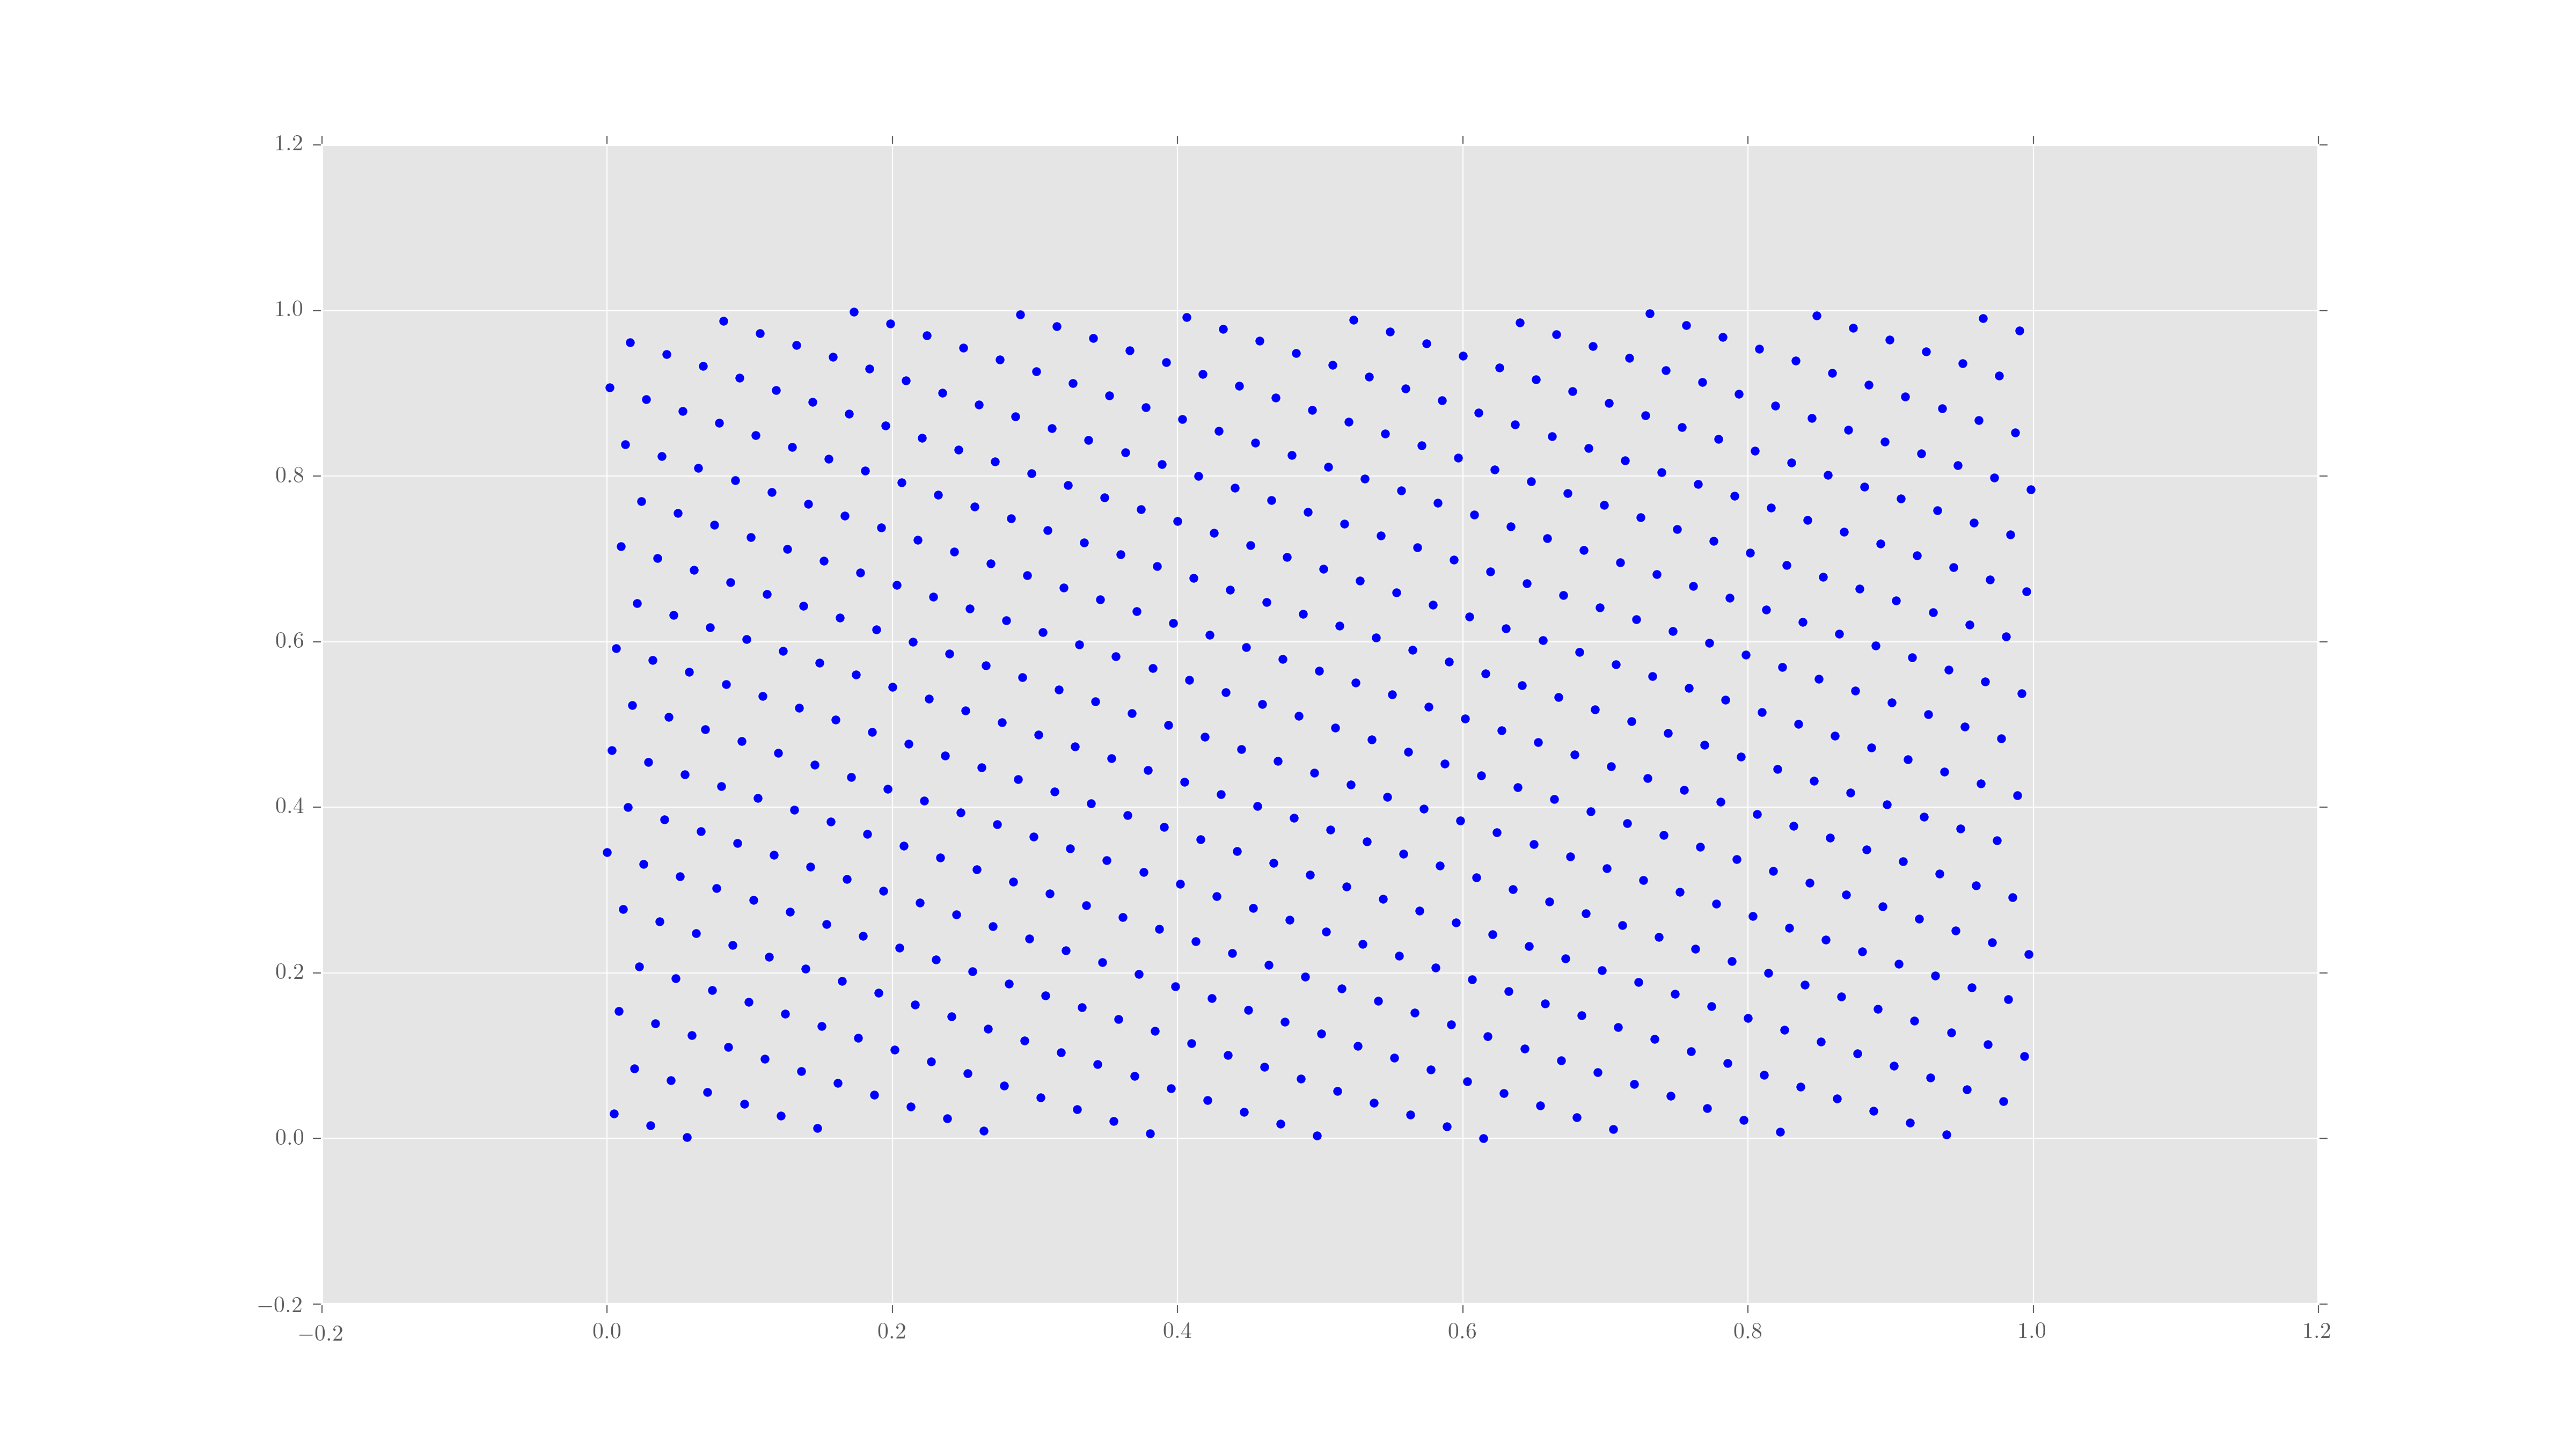
\includegraphics[width=\textwidth]{2dscatter.png}
\caption{Paare von Zufallszahlen, dargestellt als zweidimensionales Histogramm.}
\label{fig:2c1}
\end{figure}

\begin{figure}
\centering
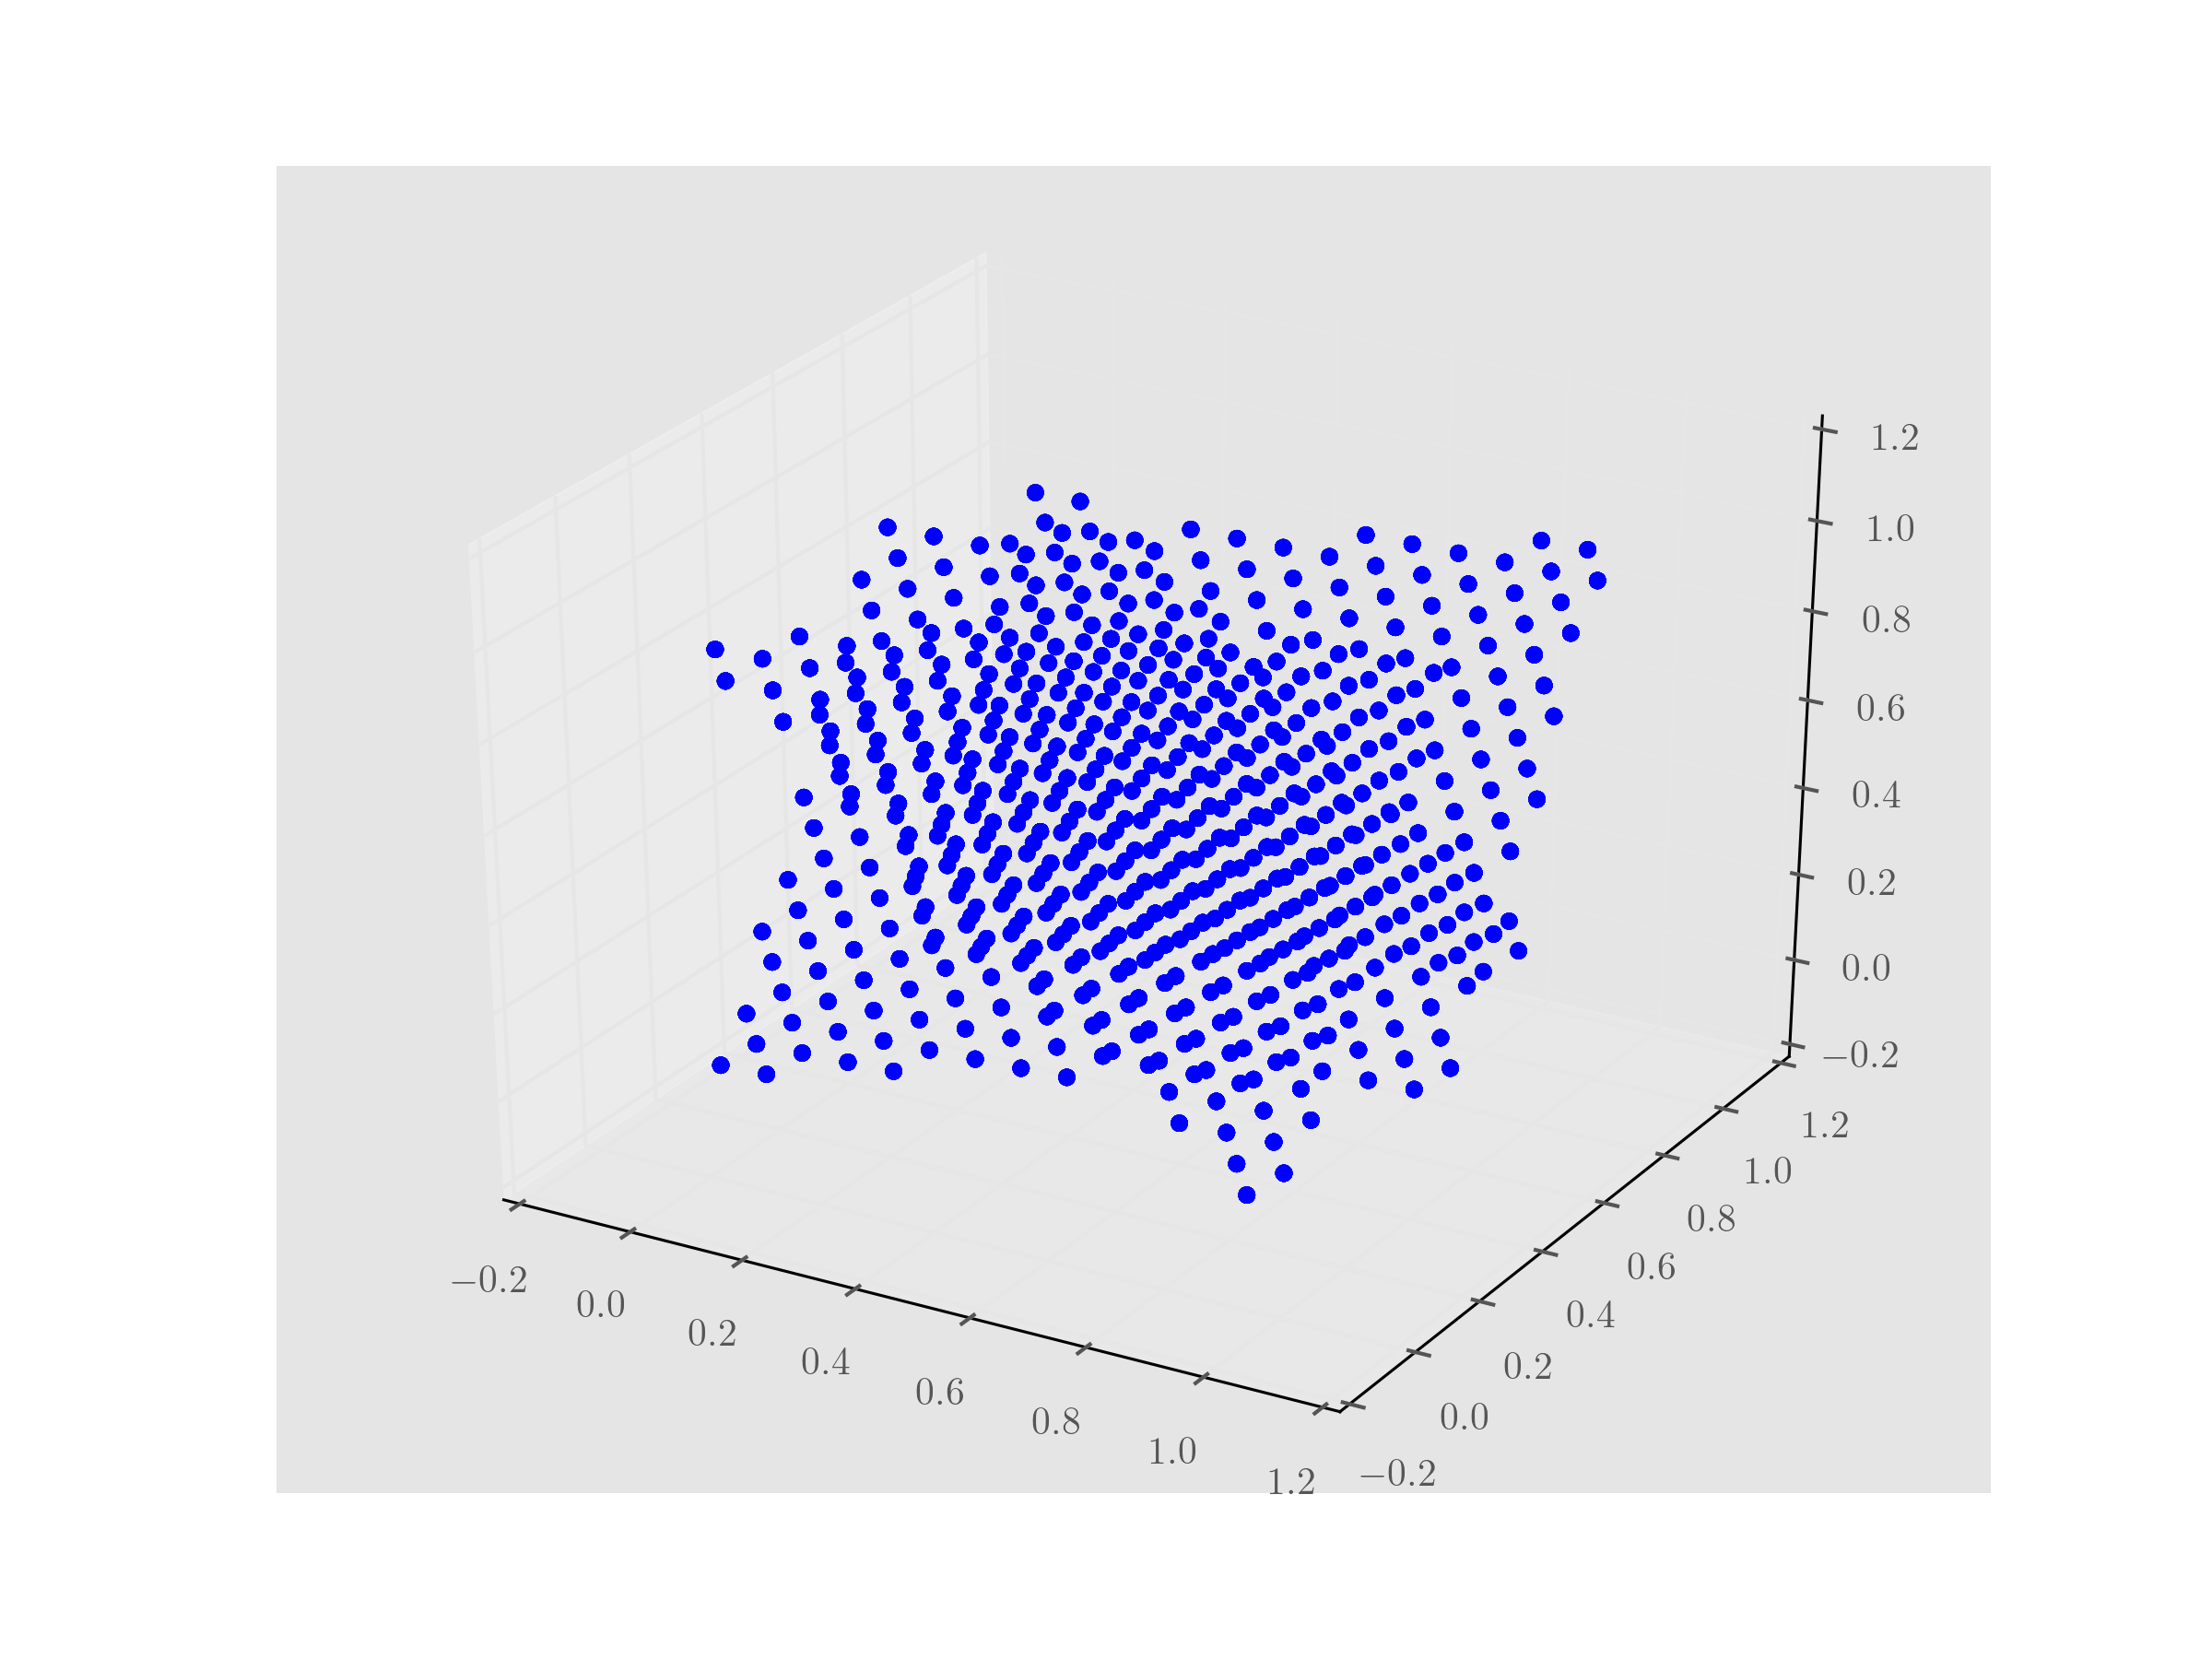
\includegraphics[width=\textwidth]{3dscatter.png}
\caption{Tripel von Zufallszahlen, dargestellt als dreidimensionales Histogramm.}
\label{fig:2c2}
\end{figure}
 

\begin{figure}
\centering
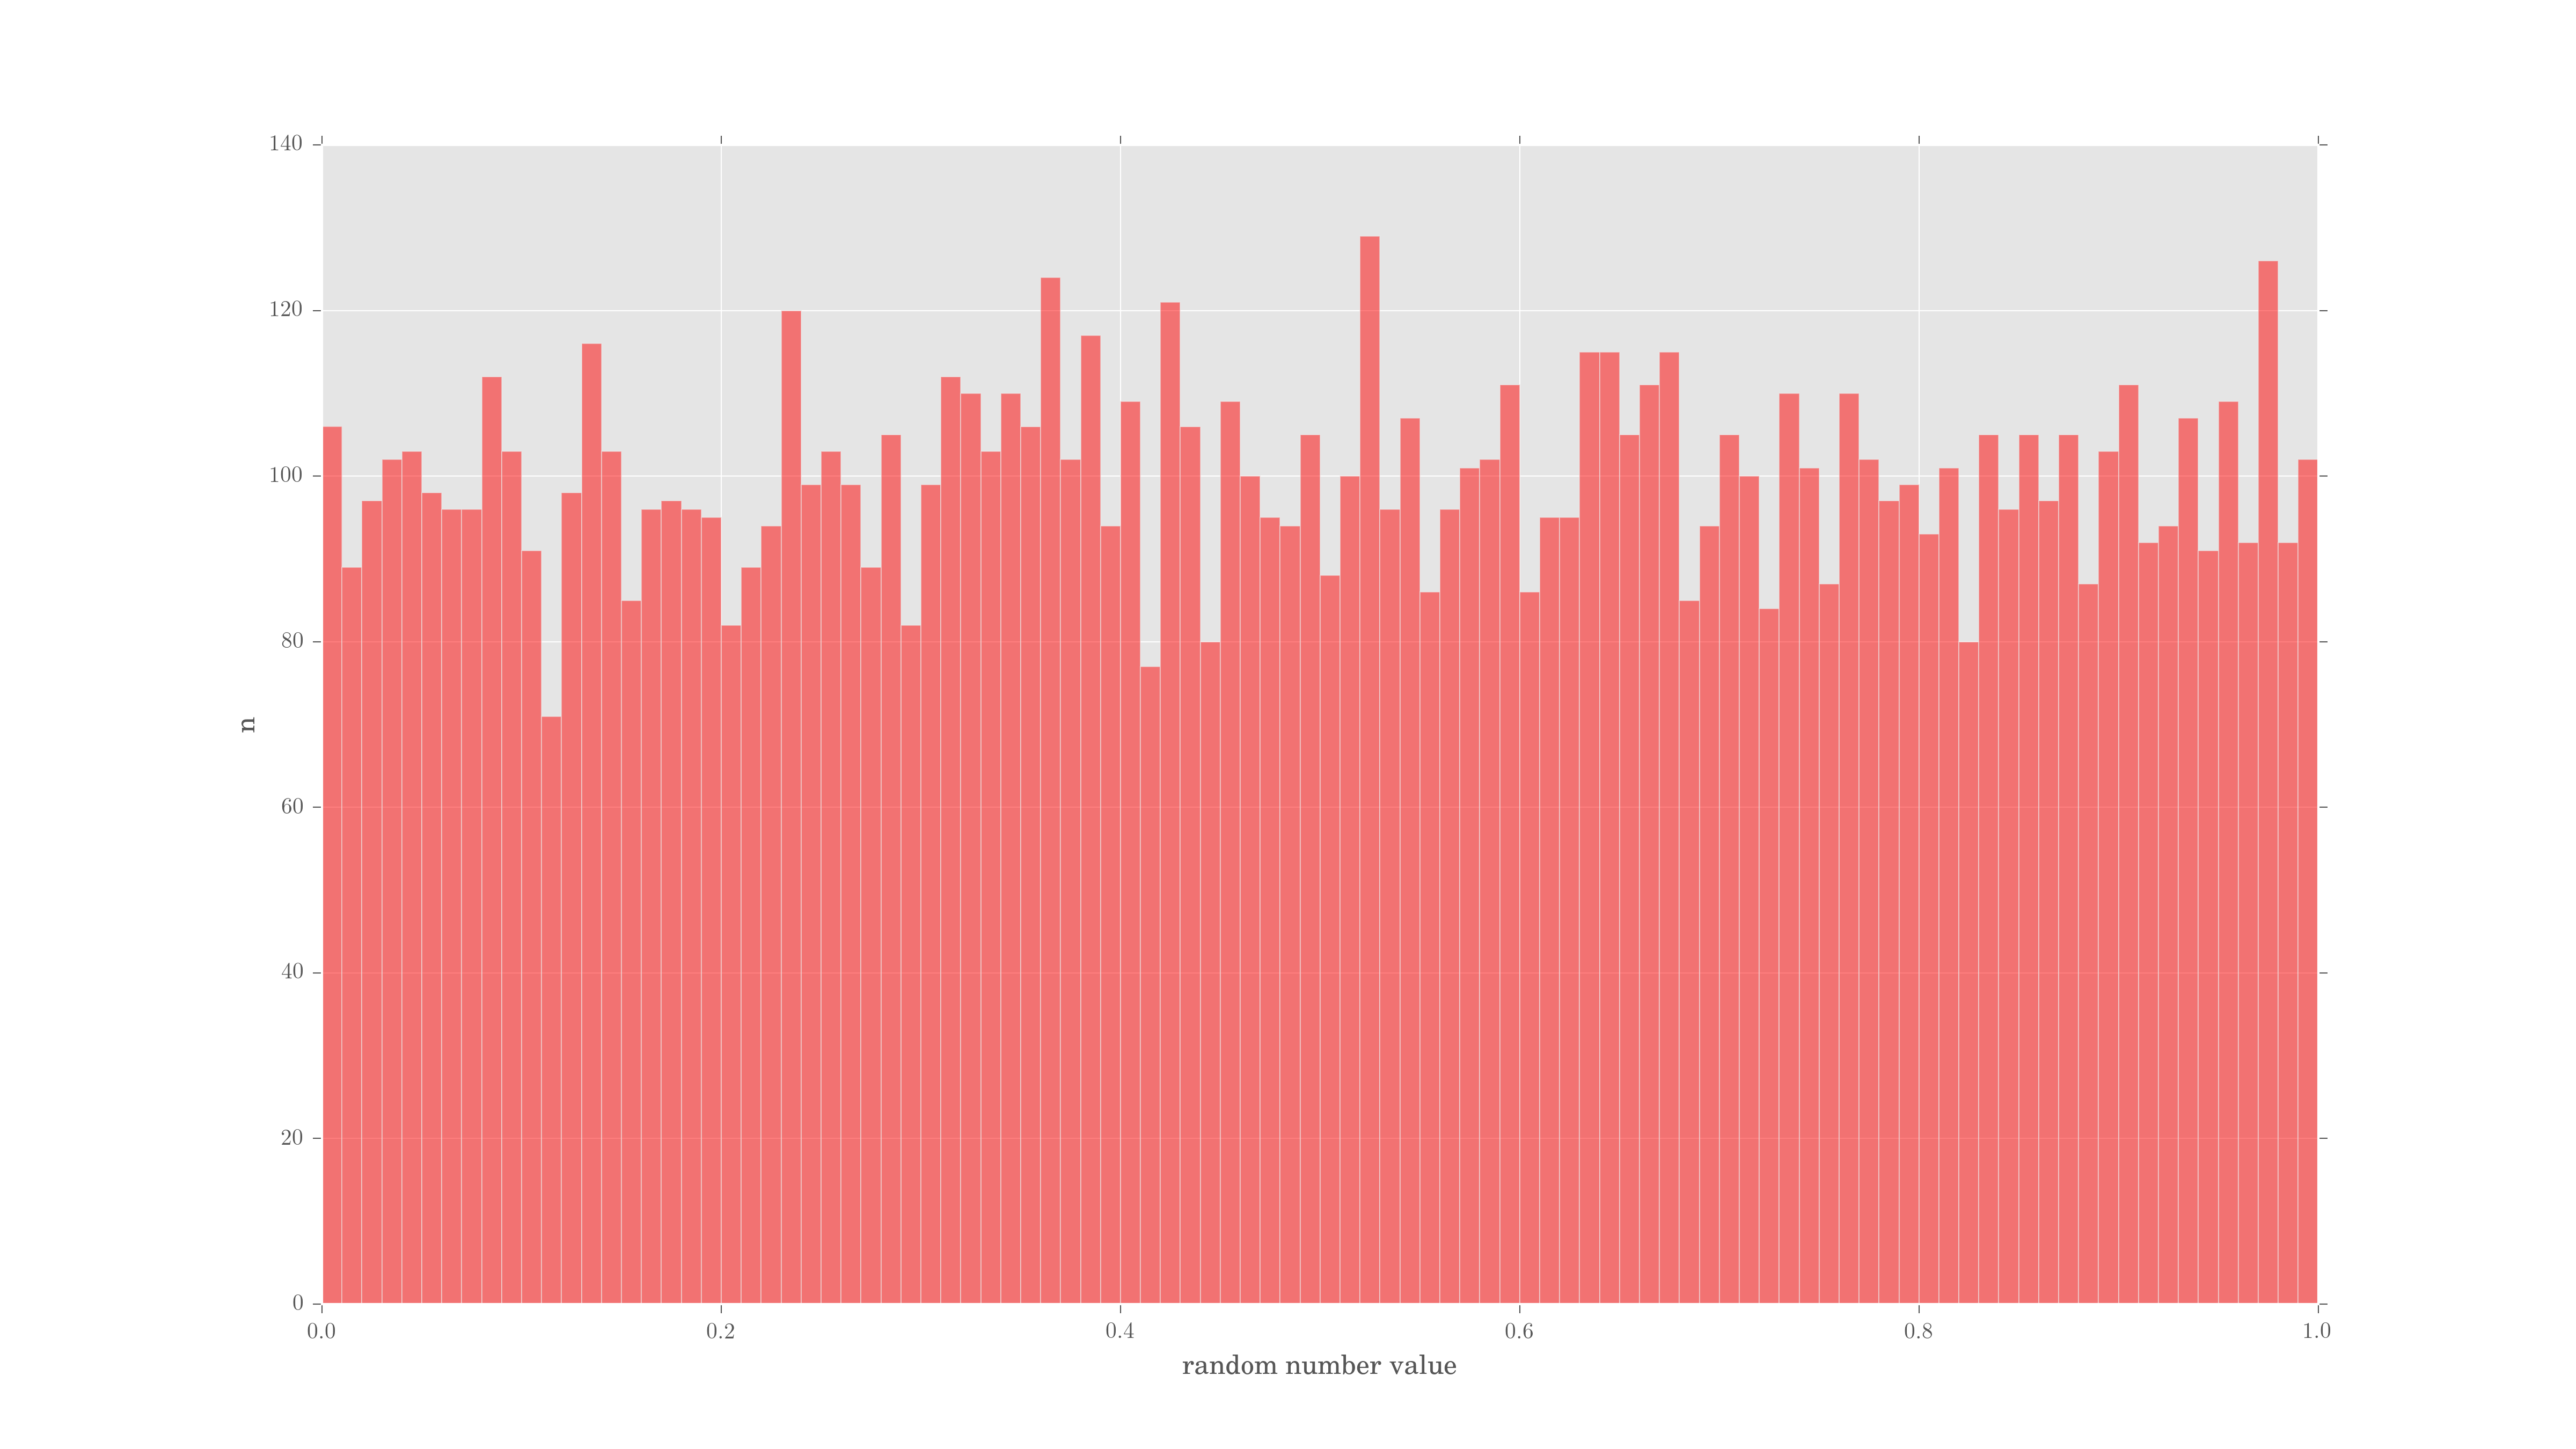
\includegraphics[width=\textwidth]{1dhist_root.png}
\caption{Mit ROOT erzeugte Zufallszahlen, dargestellt als Histogramm. Im Gegensatz zu dem vorherigen Histogramm lässt sich hier keine Struktur erkennen.}
\label{fig:2e1}
\end{figure}

\begin{figure}
\centering
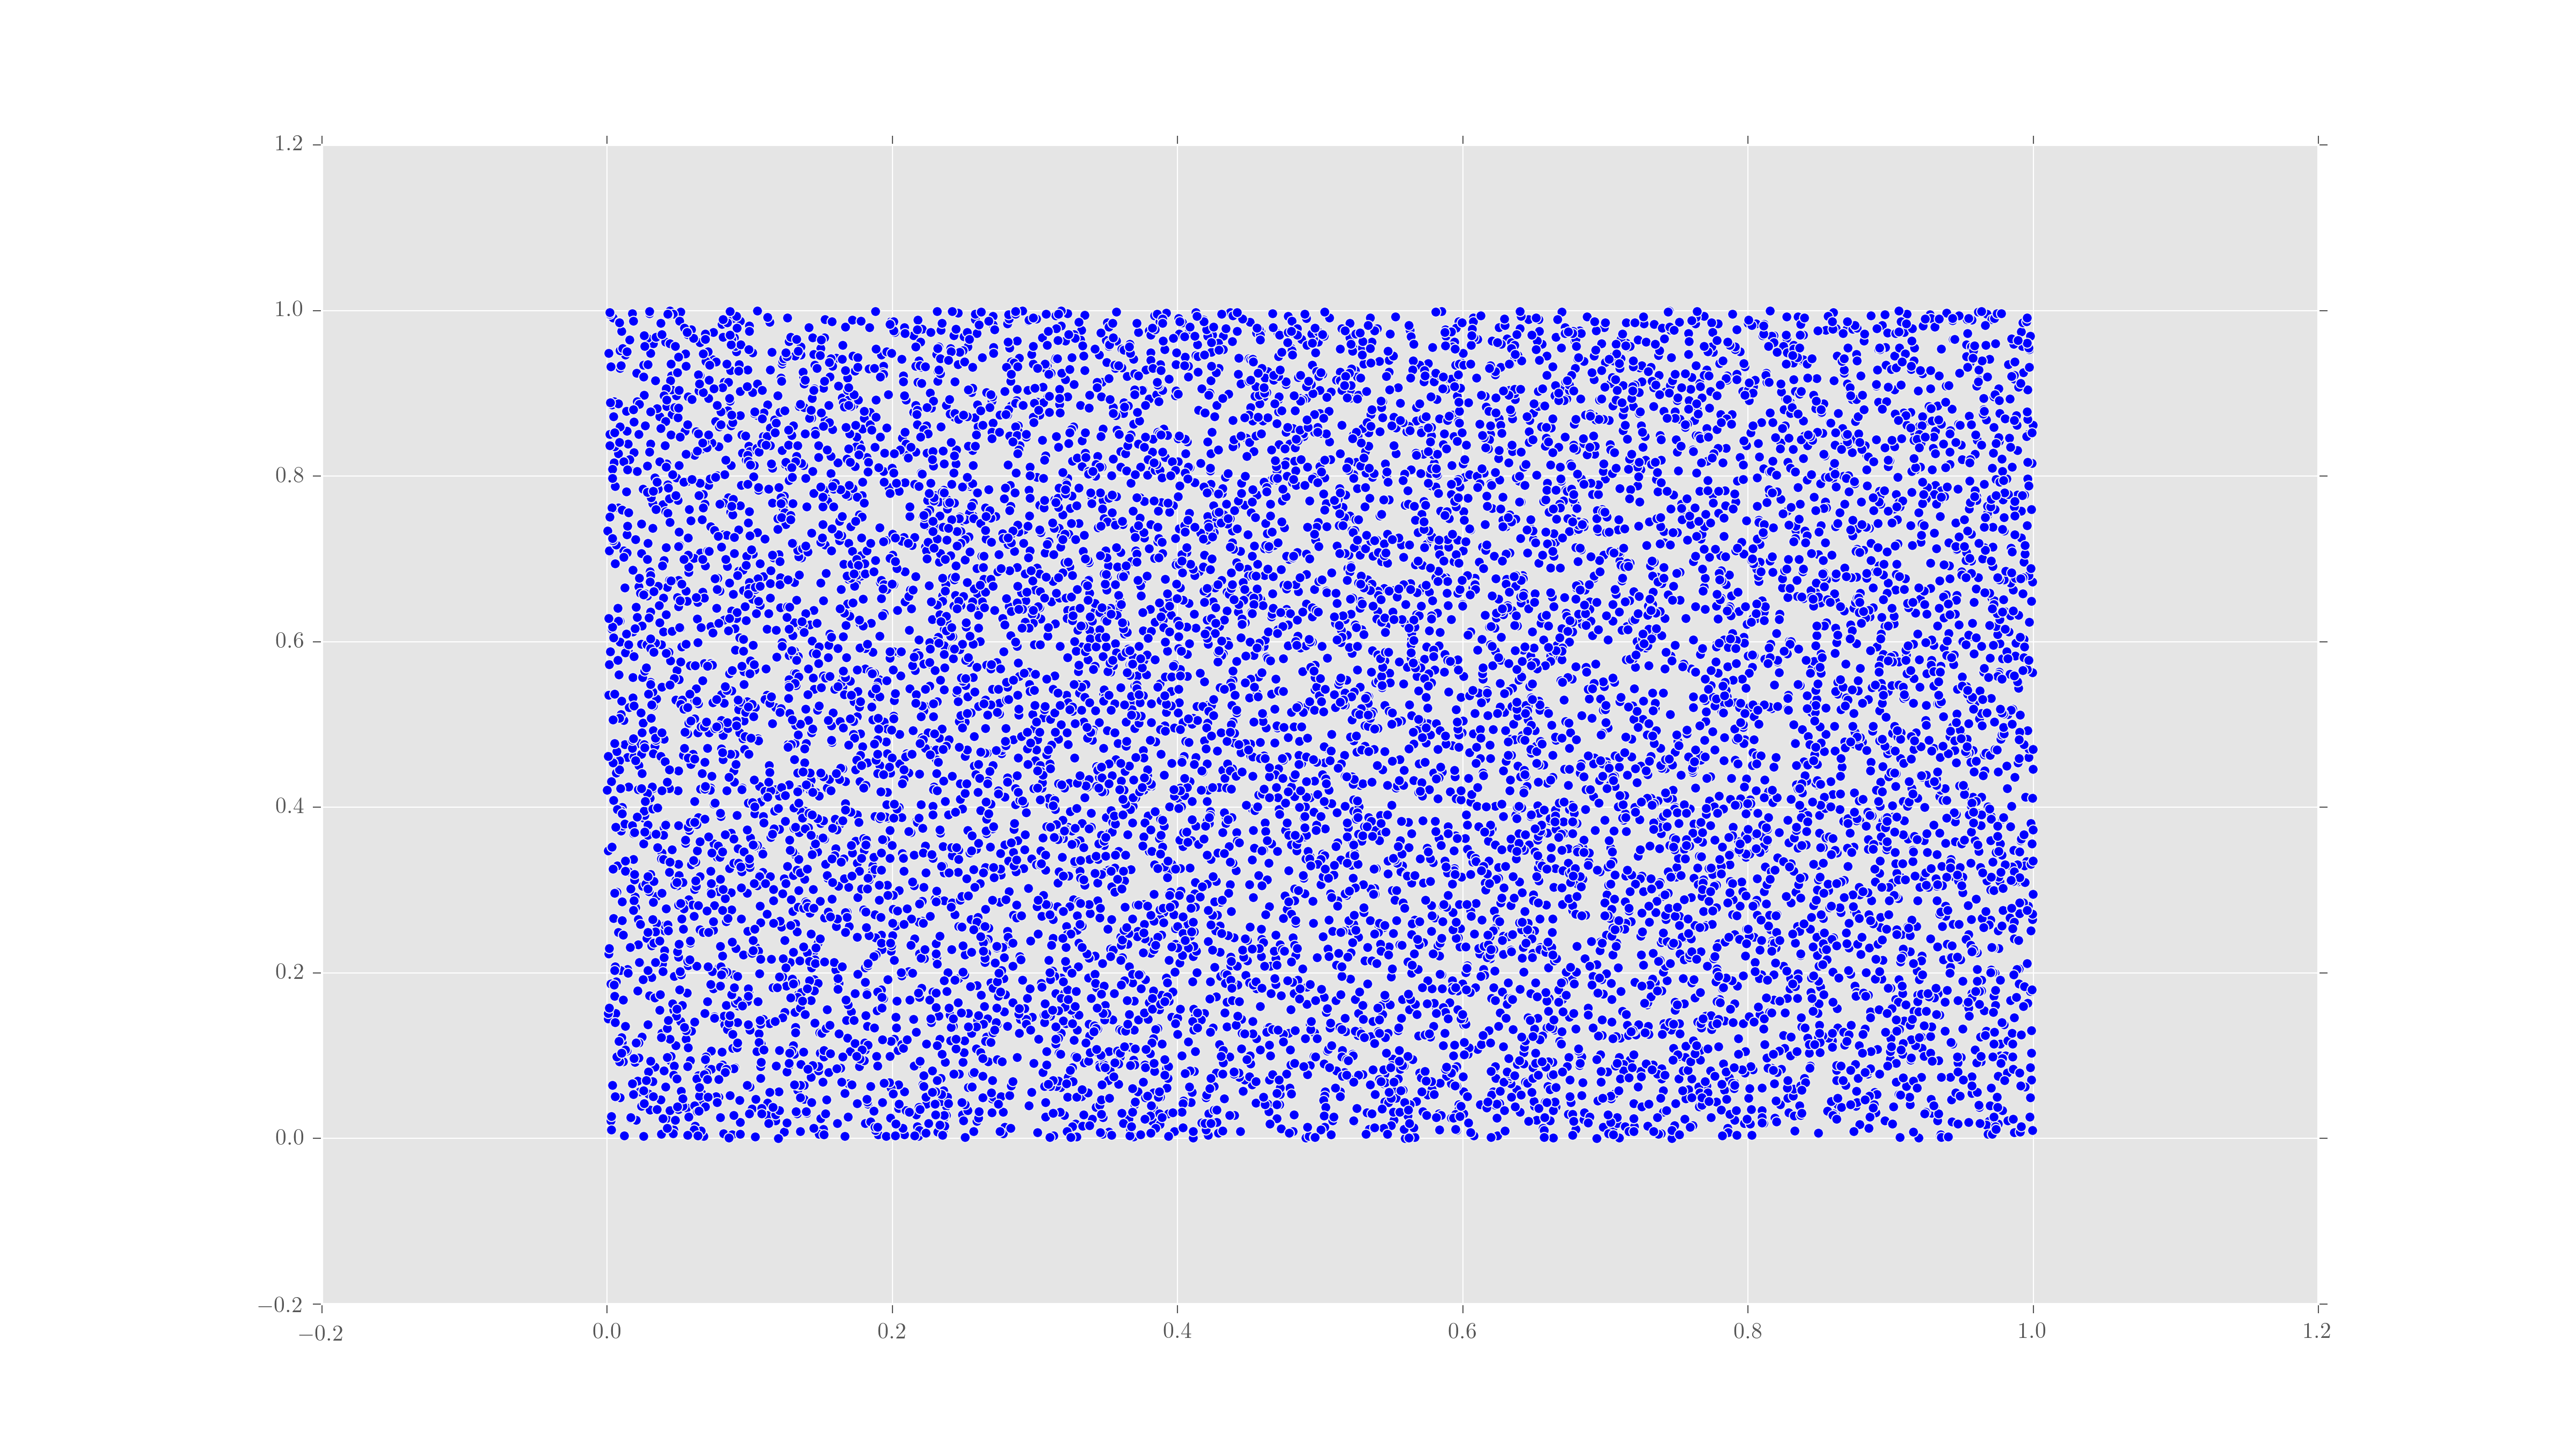
\includegraphics[width=\textwidth]{2dscatter_root.png}
\caption{Paare von Zufallszahlen, dargestellt als zweidimensionales Histogramm. Im Gegensatz zu dem vorherigen zweidimensionalen Histogramm lässt sich hier keine Struktur erkennen.}
\label{fig:2e1}
\end{figure}

\begin{figure}
\centering
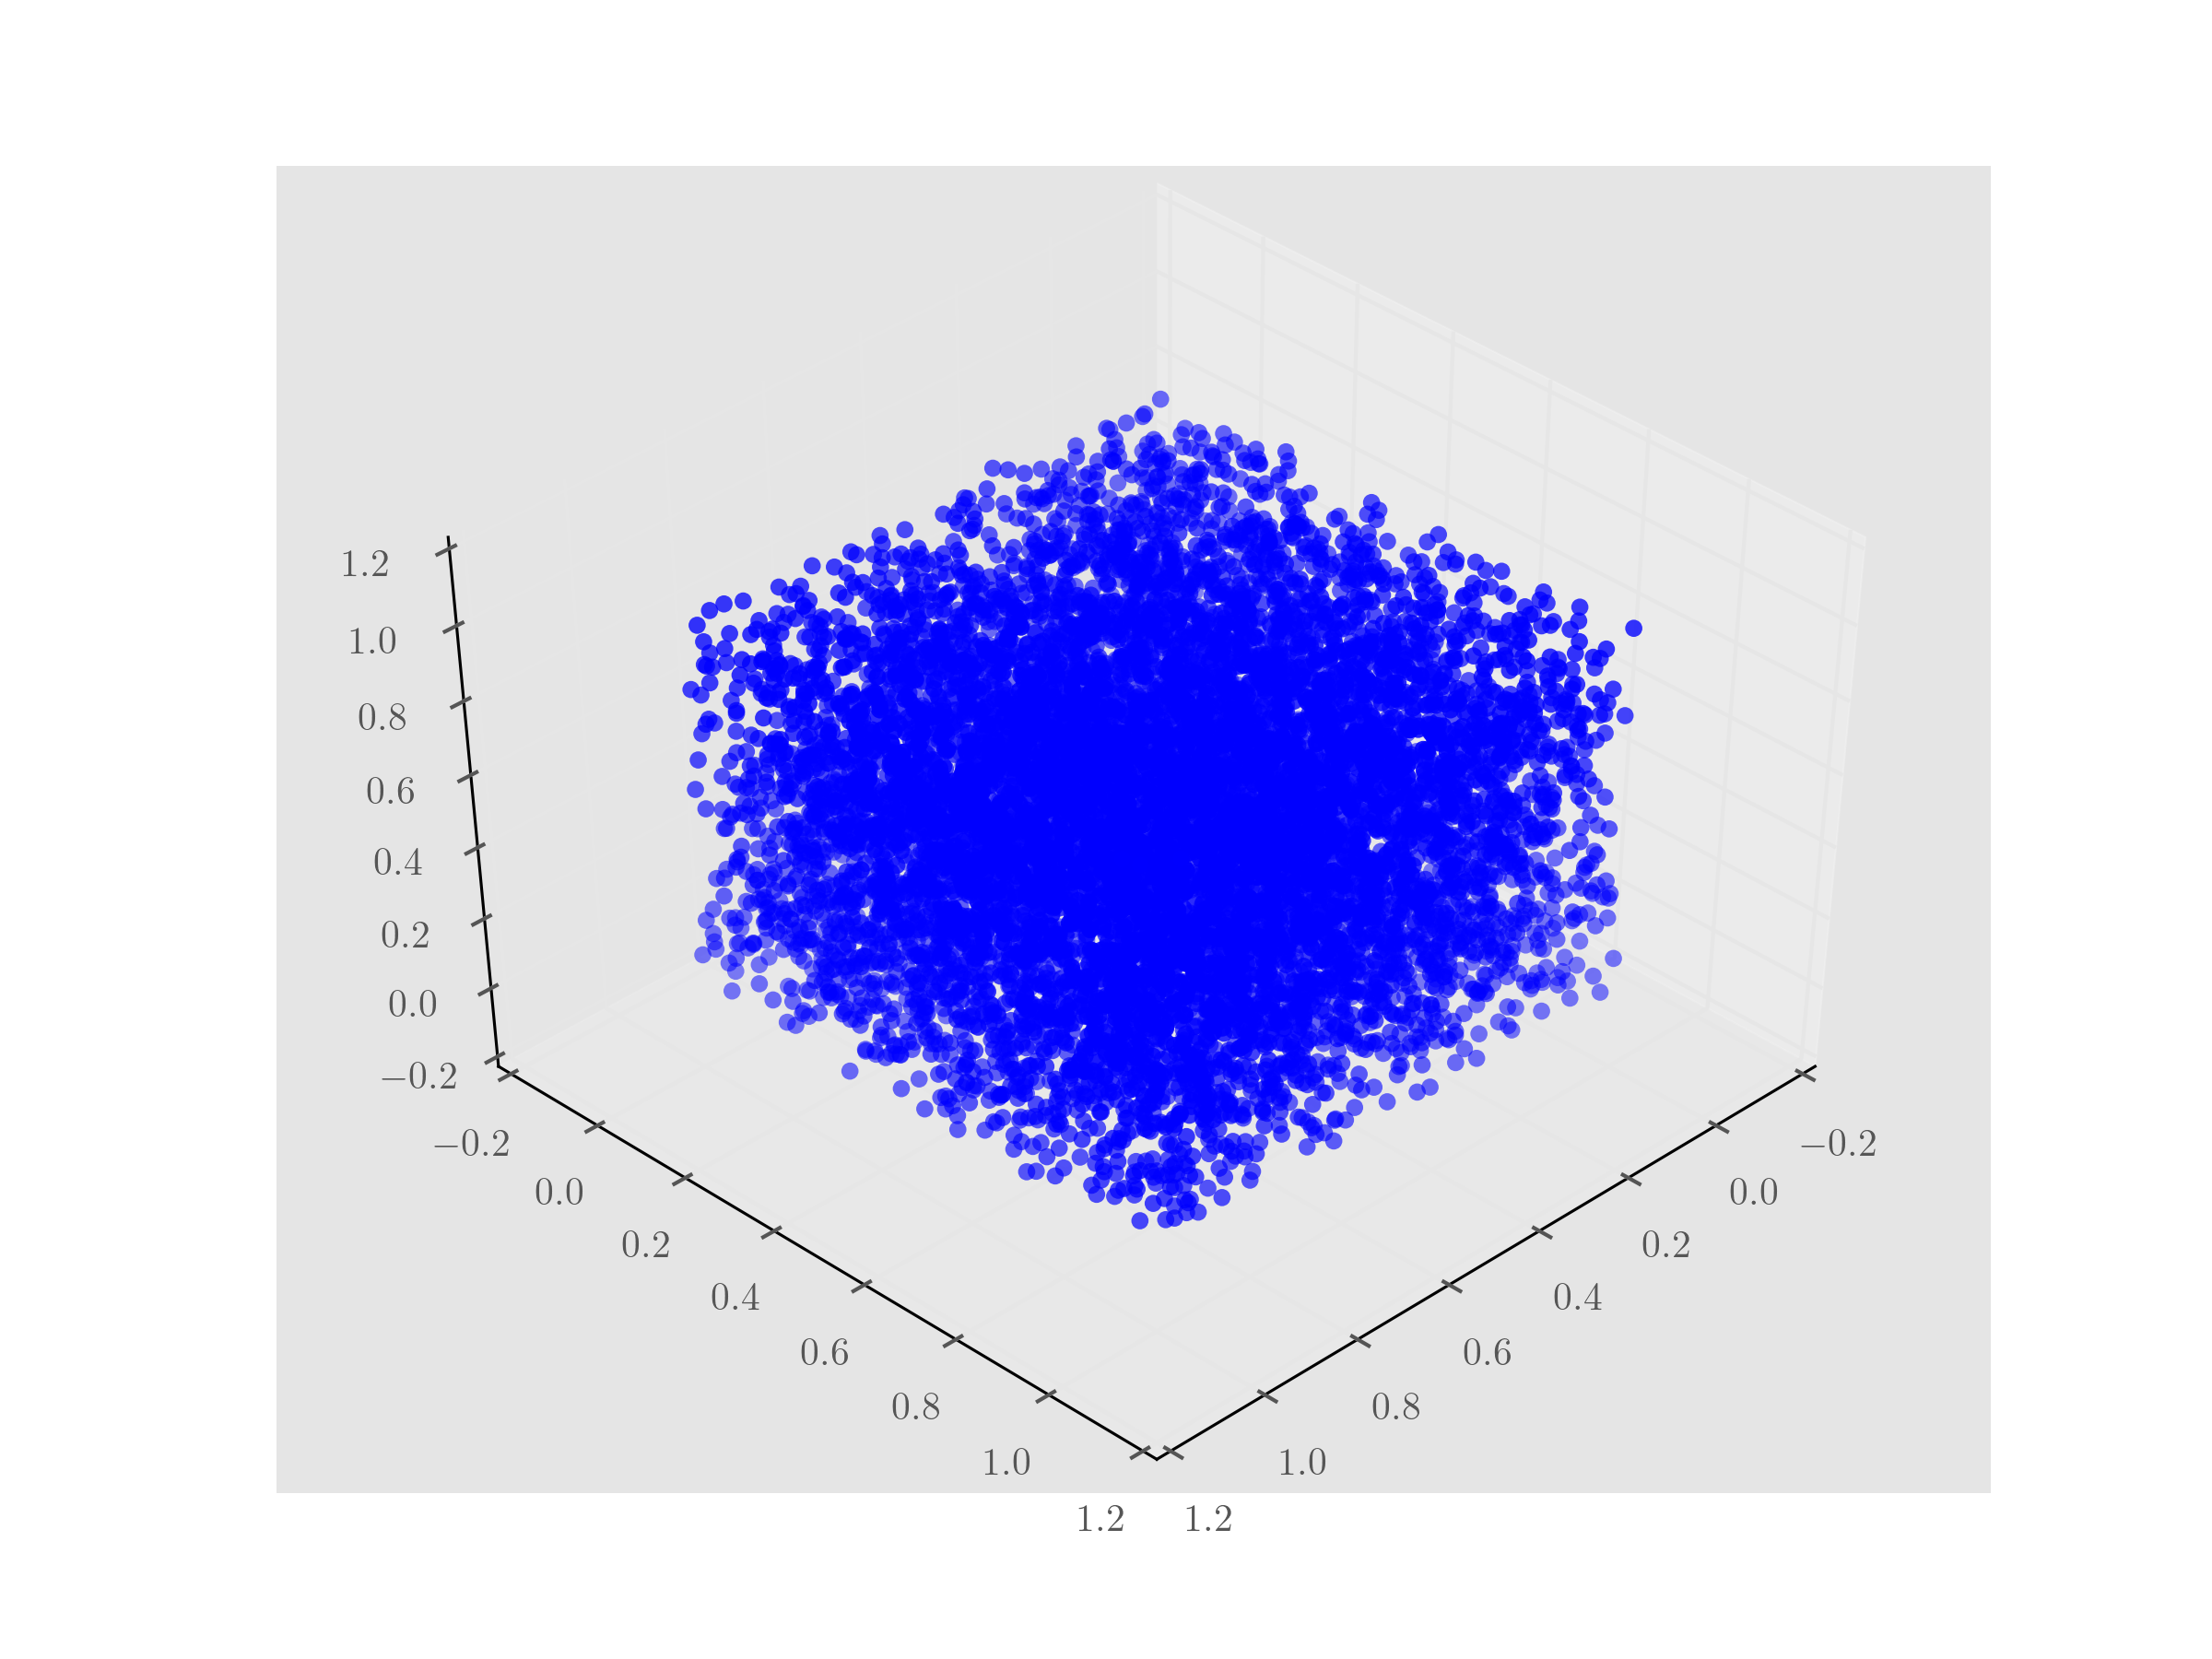
\includegraphics[width=\textwidth]{3dscatter_root.png}
\caption{Tripel von Zufallszahlen, dargestellt als dreidimensionales Histgramm.Im Gegensatz zu dem vorherigen dreidimensionalen Histogramm lassen sich hier keine Ebenen erkennen.}
\label{fig:2e2}
\end{figure}
\item[f)] Der mit den gegebenen Parametern Zufallsgenerator erzeugt nicht die Zahl $\num{0.5}$. Allerdings kann die Zahl $\num{0.5}$ erzeugt werden. Dafür wird der Algorithmus "invertiert" und es ergibt sich, dass, wenn $x_{ \text{seed} }=1144 + 10000k$ mit einer Ganzzahl $k$ , als Startwert gewählt wird die Zahl $\num{0.5}$ erzeugt wird.


\end{itemize}

\section*{Aufgabe 3: \emph{Zufallszahlengeneratoren}}
Hier werden die Transformierten Wahrscheinlichkeitsverteilungen aufgeführt.
\begin{itemize}
\item[a)]
\begin{align*}
f(x) = 1
\rightarrow x(r) =  (x_{max} - x_{min}) r + x_{min}
\end{align*}
\item[b)] 
\begin{align*}
f(t) = N e^{-t/\tau}
\rightarrow t(r) = -\tau \ln(1-r)
\end{align*}
\item[c)] 
\begin{align*}
f(x) = N x^{-n}
\rightarrow x(r) = ( r  (x_{max}^{1-n} - x_{min}^{1-n}) +x_{min}^{1-n})^{n-1}
\end{align*}
\item[d)]
\begin{align*}
f(t) = \frac{1}{\pi} \frac{1}{1+x^2}
\rightarrow x(r) = \tan\left(r-\frac{\pi}{2}\right)
\end{align*}
\end{itemize}

\section*{Aufgabe 4: \emph{Fehlerfortpflanzung}}
\begin{itemize}

\item[a)]
Mit den gegebenen Werten:
\begin{align*}
y &=a_0+a_1x \\
a_0&=a_1=1.0\pm0.2 \\
\rho& = \frac{\text{cov}(a_0,a_1)}{\sigma(a_0)\sigma(a_1)}=-0.8\\
\text{cov}(a_0,a_1)&=\rho \sigma(a_0)\sigma(a_1)=-0.8\cdot 0.2\cdot 0.2 = 0.032\\
\end{align*}
ergibt sich durch einsetzen für die Standardabweichung mit Berücksichtigung der Korrelation:
\begin{equation*}
\sigma_y = \sqrt{ 0.04 + 0.04x^2 - 0.064x }
\end{equation*}
und ohne Korrelation:
\begin{equation*}
\sigma_y = 0.2 \sqrt{1-x^2}
\end{equation*}
\item[b)] 
\begin{figure}
\centering
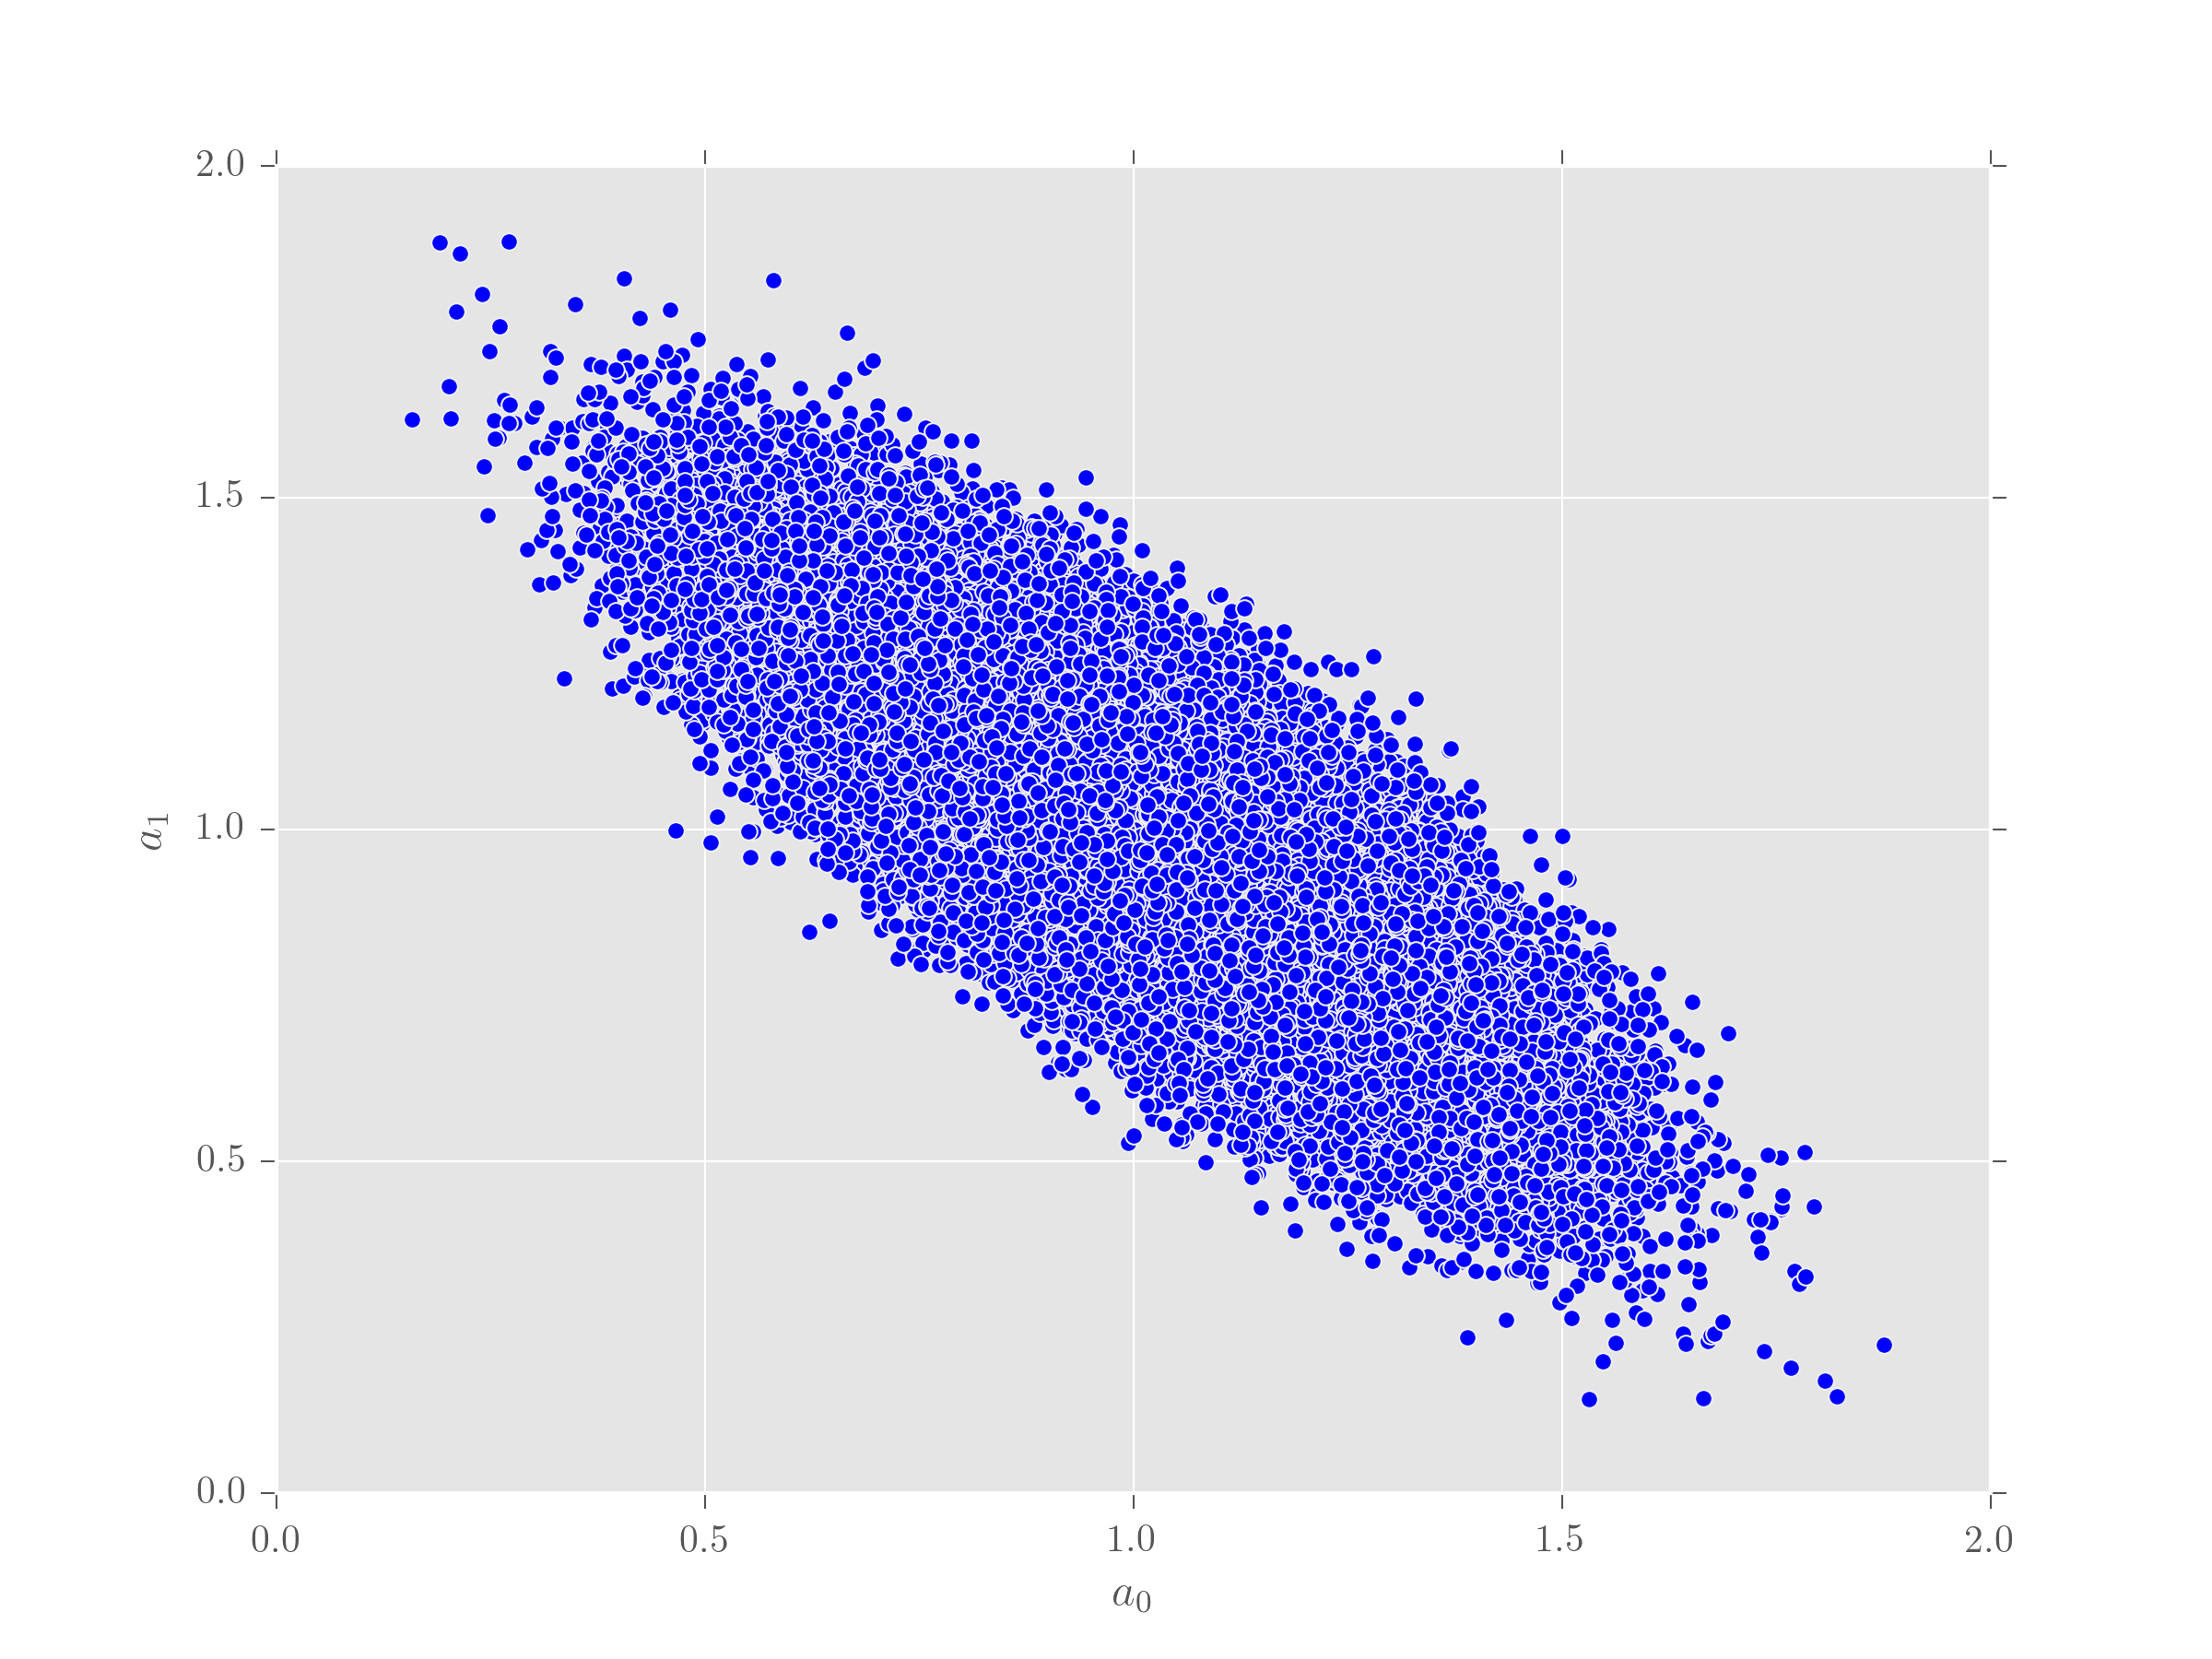
\includegraphics[width=\textwidth]{scatterplot_a0_a1.png}
\caption{Scatterplot für die Parameter $a_0$ und $a_1$ generiert durch normalverteilte Zufallszahlen mit angegebenem Mittelwert und Kovarianzmatrix.}
\label{fig:a0a1}
\end{figure}
\item[c)]
Die Vergleich von numerischer und analytischer Berechnung der Standardabweichung für $x = -3 , 0 , 3 $ liefert:
\begin{table}
\centering
\caption{Berechnung von $\sigma_y$}
\begin{tabular}{ccc}
$x$ & analytisch & numerisch \\
$-3$& $\num{0.7694}$ & $\num{0.7680}$ \\
$0$& $\num{0.2000}$ & $\num{0.1999}$ \\
$3$& $\num{0.4560}$ & $\num{0.4552}$ \\
\end{tabular}
\end{table}
Zur numerischen Berechnung wurden $\num{100000}$ Zufallszahlen verwendet.
\end{itemize}